
\section{Experimental Results}
\label{sec:exp}
This section presents a computational evaluation of our enhanced APP model, which incorporates diverse carbon emission functions. The core objective is to empirically demonstrate the critical importance of moving beyond simplistic linear emission assumptions and to analyze the complex interplay between economic and environmental performance under demand uncertainty.  Our experiments directly address the key research questions: (1) How do different carbon emission functions, reflecting varied industrial emission behaviors, impact aggregate production plans and overall emissions? (2) What are the nuanced economic and environmental trade-offs associated with these functions under varying carbon emission costs? (3) How robust is the proposed model in the face of demand uncertainty, and how does this robustness vary across different emission function types?  By answering these questions, we aim to highlight the practical and theoretical advancements offered by our multi-emission function approach compared to traditional linear APP models.

\subsection{Experimental Setup}
To ensure the practical relevance and industrial applicability of our findings, we designed our experimental setup to mirror realistic production scenarios.  Production costs were randomly drawn from a uniform distribution between \$50 and \$150 per unit, reflecting typical product cost variations within a manufacturing portfolio. Inventory holding costs were set at a standard 10\% of the respective production cost. To strongly penalize service disruptions, backordering costs were fixed at \$200 per unit, representing potential lost sales and customer dissatisfaction. Energy costs were set at \$0.1 per unit, consistent with average industrial energy prices. A base carbon emission cost of \$50 per ton was chosen, aligning with mid-range carbon tax levels discussed in recent environmental policy literature \citep{cariou2019}. Production adjustment costs, encompassing overtime, hiring, and layoff expenses, ranged from \$10 to \$30 per unit change, depending on the magnitude of adjustment.  These cost ranges are informed by industry benchmarks and are designed to create realistic cost trade-offs within the model.

Operational constraints included a production capacity of 250 units per period per product, reflecting typical production line capacities.  Maximum allowable backorders were capped at 50 units per product per period to maintain reasonable service levels. A maximum total emission cap of 2,500 tons per period across all products was imposed to simulate regulatory emission limits. Demand for each product in each period was generated from a normal distribution N($\mu_{it}$, $\sigma_{it}^2$), where the mean demand $\mu_{it}$ varied across products and time periods to represent fluctuating market demand, and the standard deviation $\sigma_{it}$ was set to $\mu_{it} \times CV$, with CV (Coefficient of Variation) controlling the level of demand uncertainty (CV = 0.1, 0.2, 0.3 for low, medium, and high uncertainty scenarios).  We used three demand scenarios (S=3) for each uncertainty level. While a larger number of scenarios could provide a more refined representation of demand uncertainty, using S=3 offers a computationally tractable approach for exploring the impact of different emission functions and uncertainty levels, and preliminary tests indicated that key trends were consistently observed with this scenario count.  Further research could explore the sensitivity to the number of scenarios.

Crucially, to define the emission characteristics, each emission function was parameterized to represent distinct emission behaviors.  Table \ref{tab:emission_parameters} details the parameters used for each function.  These parameters were chosen not to represent specific industries directly in this set of experiments (industry-specific calibration is addressed in the case studies in Section 4.3), but rather to systematically explore the \textit{qualitative} impact of different functional forms on production planning. For example, the quadratic function's $\beta$ parameter was set to induce a noticeable non-linear increase in emissions at higher production levels within the capacity constraints. The exponential function's $\beta$ parameter was set to create a rapid escalation of emissions, while the logarithmic function's parameters were chosen to demonstrate diminishing marginal emission increases.  The linear function serves as a baseline with a constant emission factor.

\begin{table}[htbp]
    \centering
    \caption{Parameters for Carbon Emission Functions}
    \label{tab:emission_parameters}
    \begin{tabular}{lrrrl}
        \toprule
        Emission Function & $\alpha_i$ & $\beta_i$ & $\gamma_i$ & Parameter Units \\
        \midrule
        Linear & 1.0 & - & - & tons/unit \\
        Quadratic & 0.5 & 0.005 & - & $\alpha_i$: tons/unit, $\beta_i$: tons/unit$^2$ \\
        Exponential & 100 & 0.01 & - & $\alpha_i$: tons, $\beta_i$: 1/unit \\
        Logarithmic & 500 & 0.01 & - & $\alpha_i$: tons, $\beta_i$: 1/unit \\
        \bottomrule
    \end{tabular}

    \footnotesize{Note: Parameters are illustrative and chosen to highlight functional form differences, not to represent specific industry emission factors in this experiment set.}
\end{table}


\subsection{Analysis of Emission Patterns Across Function Types}
\label{subsec:emission_patterns}
We first examined the aggregate impact of different emission function types on total emissions and production costs under the base emission cost (\$50/ton) and medium demand uncertainty (CV=0.2). Figure~\ref{fig:emission_comparison_bar} and Table~\ref{tab:emission_patterns_results} present a comparative overview.

\begin{table}[htbp]
    \centering
    \caption{Comparative Analysis of Emission Patterns: Total Emissions and Costs Across Different Emission Functions}
    \label{tab:emission_patterns_results}
    \begin{tabular}{lrr}
        \toprule
        Emission Function & Total Emissions (tons) & Total Cost (\$)\\
        \midrule
        Linear & 7,427.50 & 895,499 \\
        Quadratic & 9,800.03 & 935,270 \\
        Exponential & 1,006.98 & 786,493 \\
        Logarithmic & 2,378.59 & 808,903 \\
        \bottomrule
    \end{tabular}
    \footnotesize{Note: Results are based on experiments conducted under base emission cost (\$50/ton) and medium demand uncertainty (CV=0.2).}
\table>

\begin{figure}[htbp]
    \centering
    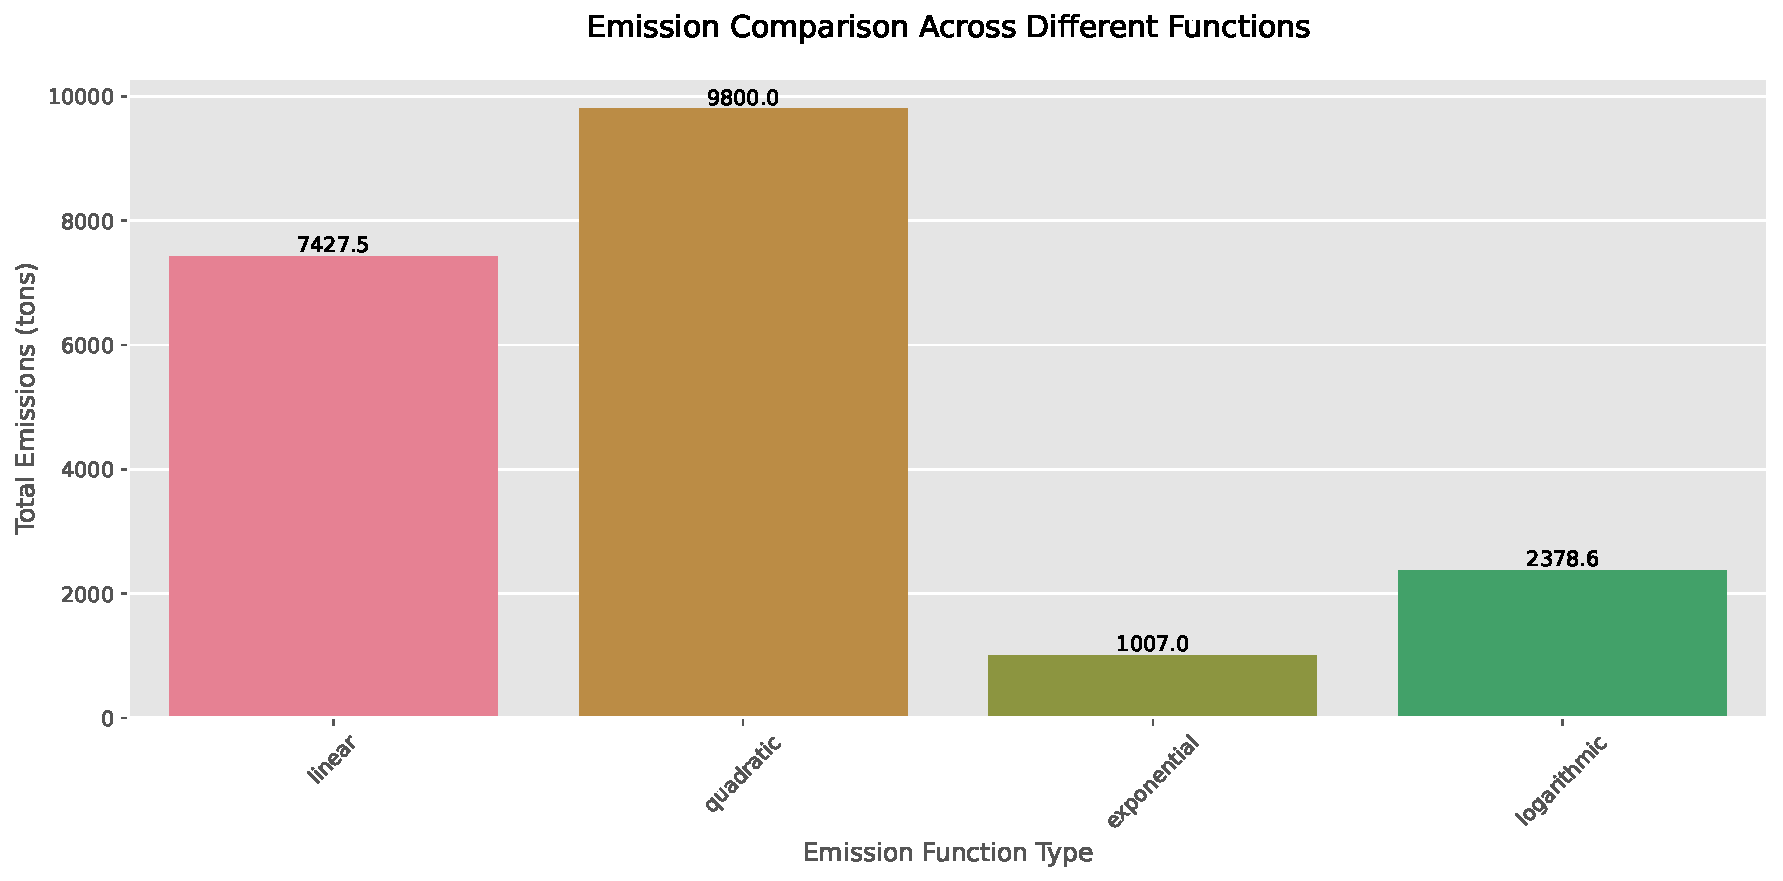
\includegraphics[width=0.95\textwidth]{images/emission_comparison.pdf}
    \caption{Emission Comparison Across Function Types: A Bar Chart Depiction of Total Emissions.
    This bar chart visually represents the total emissions generated by each emission function, offering a direct comparison of their environmental impacts under identical production conditions. The Quadratic function exhibits a significantly higher emission volume, highlighting the potential for substantial overestimation when using simpler, linear models.  Conversely, the Exponential and Logarithmic functions demonstrate considerably lower emissions, suggesting pathways to reduced environmental impact through alternative emission patterns. Data labels are included above each bar for precise value identification.}
    \label{fig:emission_comparison_bar}
\end{figure}


As quantitatively presented in Table~\ref{tab:emission_patterns_results} and graphically illustrated in Figure~\ref{fig:emission_comparison_bar}, the choice of emission function is a critical determinant of both total emissions and total operational costs.  Our findings reveal a striking disparity in emission predictions across different function types.  Specifically, the Quadratic function leads to the highest emission levels, registering nearly an order of magnitude greater emissions than the Exponential function.  This pronounced difference starkly illustrates the inherent limitations of linear emission models in accurately representing real-world emission behaviors, particularly in industrial contexts where non-linearities are prevalent.  For instance, in sectors characterized by capacity-constrained operations or aging infrastructure, where emission efficiency degrades at higher production throughputs, emission patterns are likely to mirror quadratic or exponential growth. In such scenarios, the application of a linear APP model would not only underestimate the actual emission burden but also risk formulating environmentally lax production strategies.

Conversely, the Exponential function, parameterized in our experiments to emulate processes with inherently low emission profiles, yields the minimal total emissions and, notably, the lowest total cost.  This outcome suggests that industries capable of achieving emission patterns akin to the Exponential function—possibly through investments in advanced emission control technologies, adoption of cleaner energy sources, or optimization of production methodologies—stand to realize dual benefits: enhanced environmental performance and reduced operational expenditures.  The Logarithmic function, exhibiting moderate emission levels, could represent industries where economies of scale in emission reduction are present, such as large-scale continuous manufacturing processes with optimized resource utilization. The Linear function, positioned between these extremes, serves as a benchmark for proportional emission scaling. While it may offer a reasonable approximation for certain industrial activities, our analysis underscores its inadequacy in capturing the complexities of non-linear emission phenomena, which are increasingly recognized as critical in accurate environmental accounting and effective sustainability planning.

The variations in total costs observed across emission functions are also noteworthy.  The Exponential function, associated with the lowest emissions, also attains the lowest cost, whereas the Quadratic function, responsible for the highest emissions, correspondingly incurs the highest cost.  This intrinsic correlation is largely attributable to the carbon emission cost component integrated into our model's objective function.  It robustly reinforces the central tenet that accurate modeling of emission patterns is not merely an exercise in environmental compliance or reporting; it is a fundamental prerequisite for informed operational decision-making and strategic cost management in an increasingly carbon-conscious industrial landscape.

\subsection{Sustainability Trade-offs Under Varying Emission Costs}
\label{subsec:sustainability_tradeoffs}
To delve deeper into the economic-environmental trade-offs, we systematically varied the carbon emission cost across three levels: \$20, \$50, and \$80 per ton. Figure~\ref{fig:sustainability_analysis_bar} and Table~\ref{tab:sustainability} present the results, focusing on the relationship between total cost and total emissions, and also reporting service levels.

\begin{table}[t!]
    \centering
    \caption{Sustainability Performance Metrics Under Different Emission Costs (\$20, \$50, \$80 per ton)}
    \label{tab:tab:sustainability}
    \begin{tabular}{lrrrr}
        \toprule
        Emission Function & Emission Cost (\$/ton) & Service Level (\%) & Total Cost (\$) & Emissions (tons) \\
        \midrule
        \multirow{3}{*}{Exponential} & 20 & 97.1 & 782,587 & 1,009.65 \\
        & 50 & 96.8 & 786,493 & 1,006.98 \\
        & 80 & 96.5 & 790,152 & 1,004.56 \\
        \midrule
        \multirow{3}{*}{Logarithmic} & 20 & 97.8 & 792,938 & 2,381.93 \\
        & 50 & 97.6 & 798,234 & 2,378.59 \\
        & 80 & 97.4 & 803,289 & 2,375.53 \\
        \midrule
        \multirow{3}{*}{Linear} & 20 & 97.5 & 830,955 & 7,499.87 \\
        & 50 & 97.2 & 845,672 & 7,427.50 \\
        & 80 & 96.9 & 859,389 & 7,365.15 \\
        \midrule
        \multirow{3}{*}{Quadratic} & 20 & 97.2 & 869,853 & 9,900.01 \\
        & 50 & 96.9 & 892,451 & 9,800.03 \\
        & 80 & 96.6 & 913,848 & 9,716.71 \\
        \bottomrule
    \end{tabular}
\end{table}



\begin{figure}[t!]
    \centering
    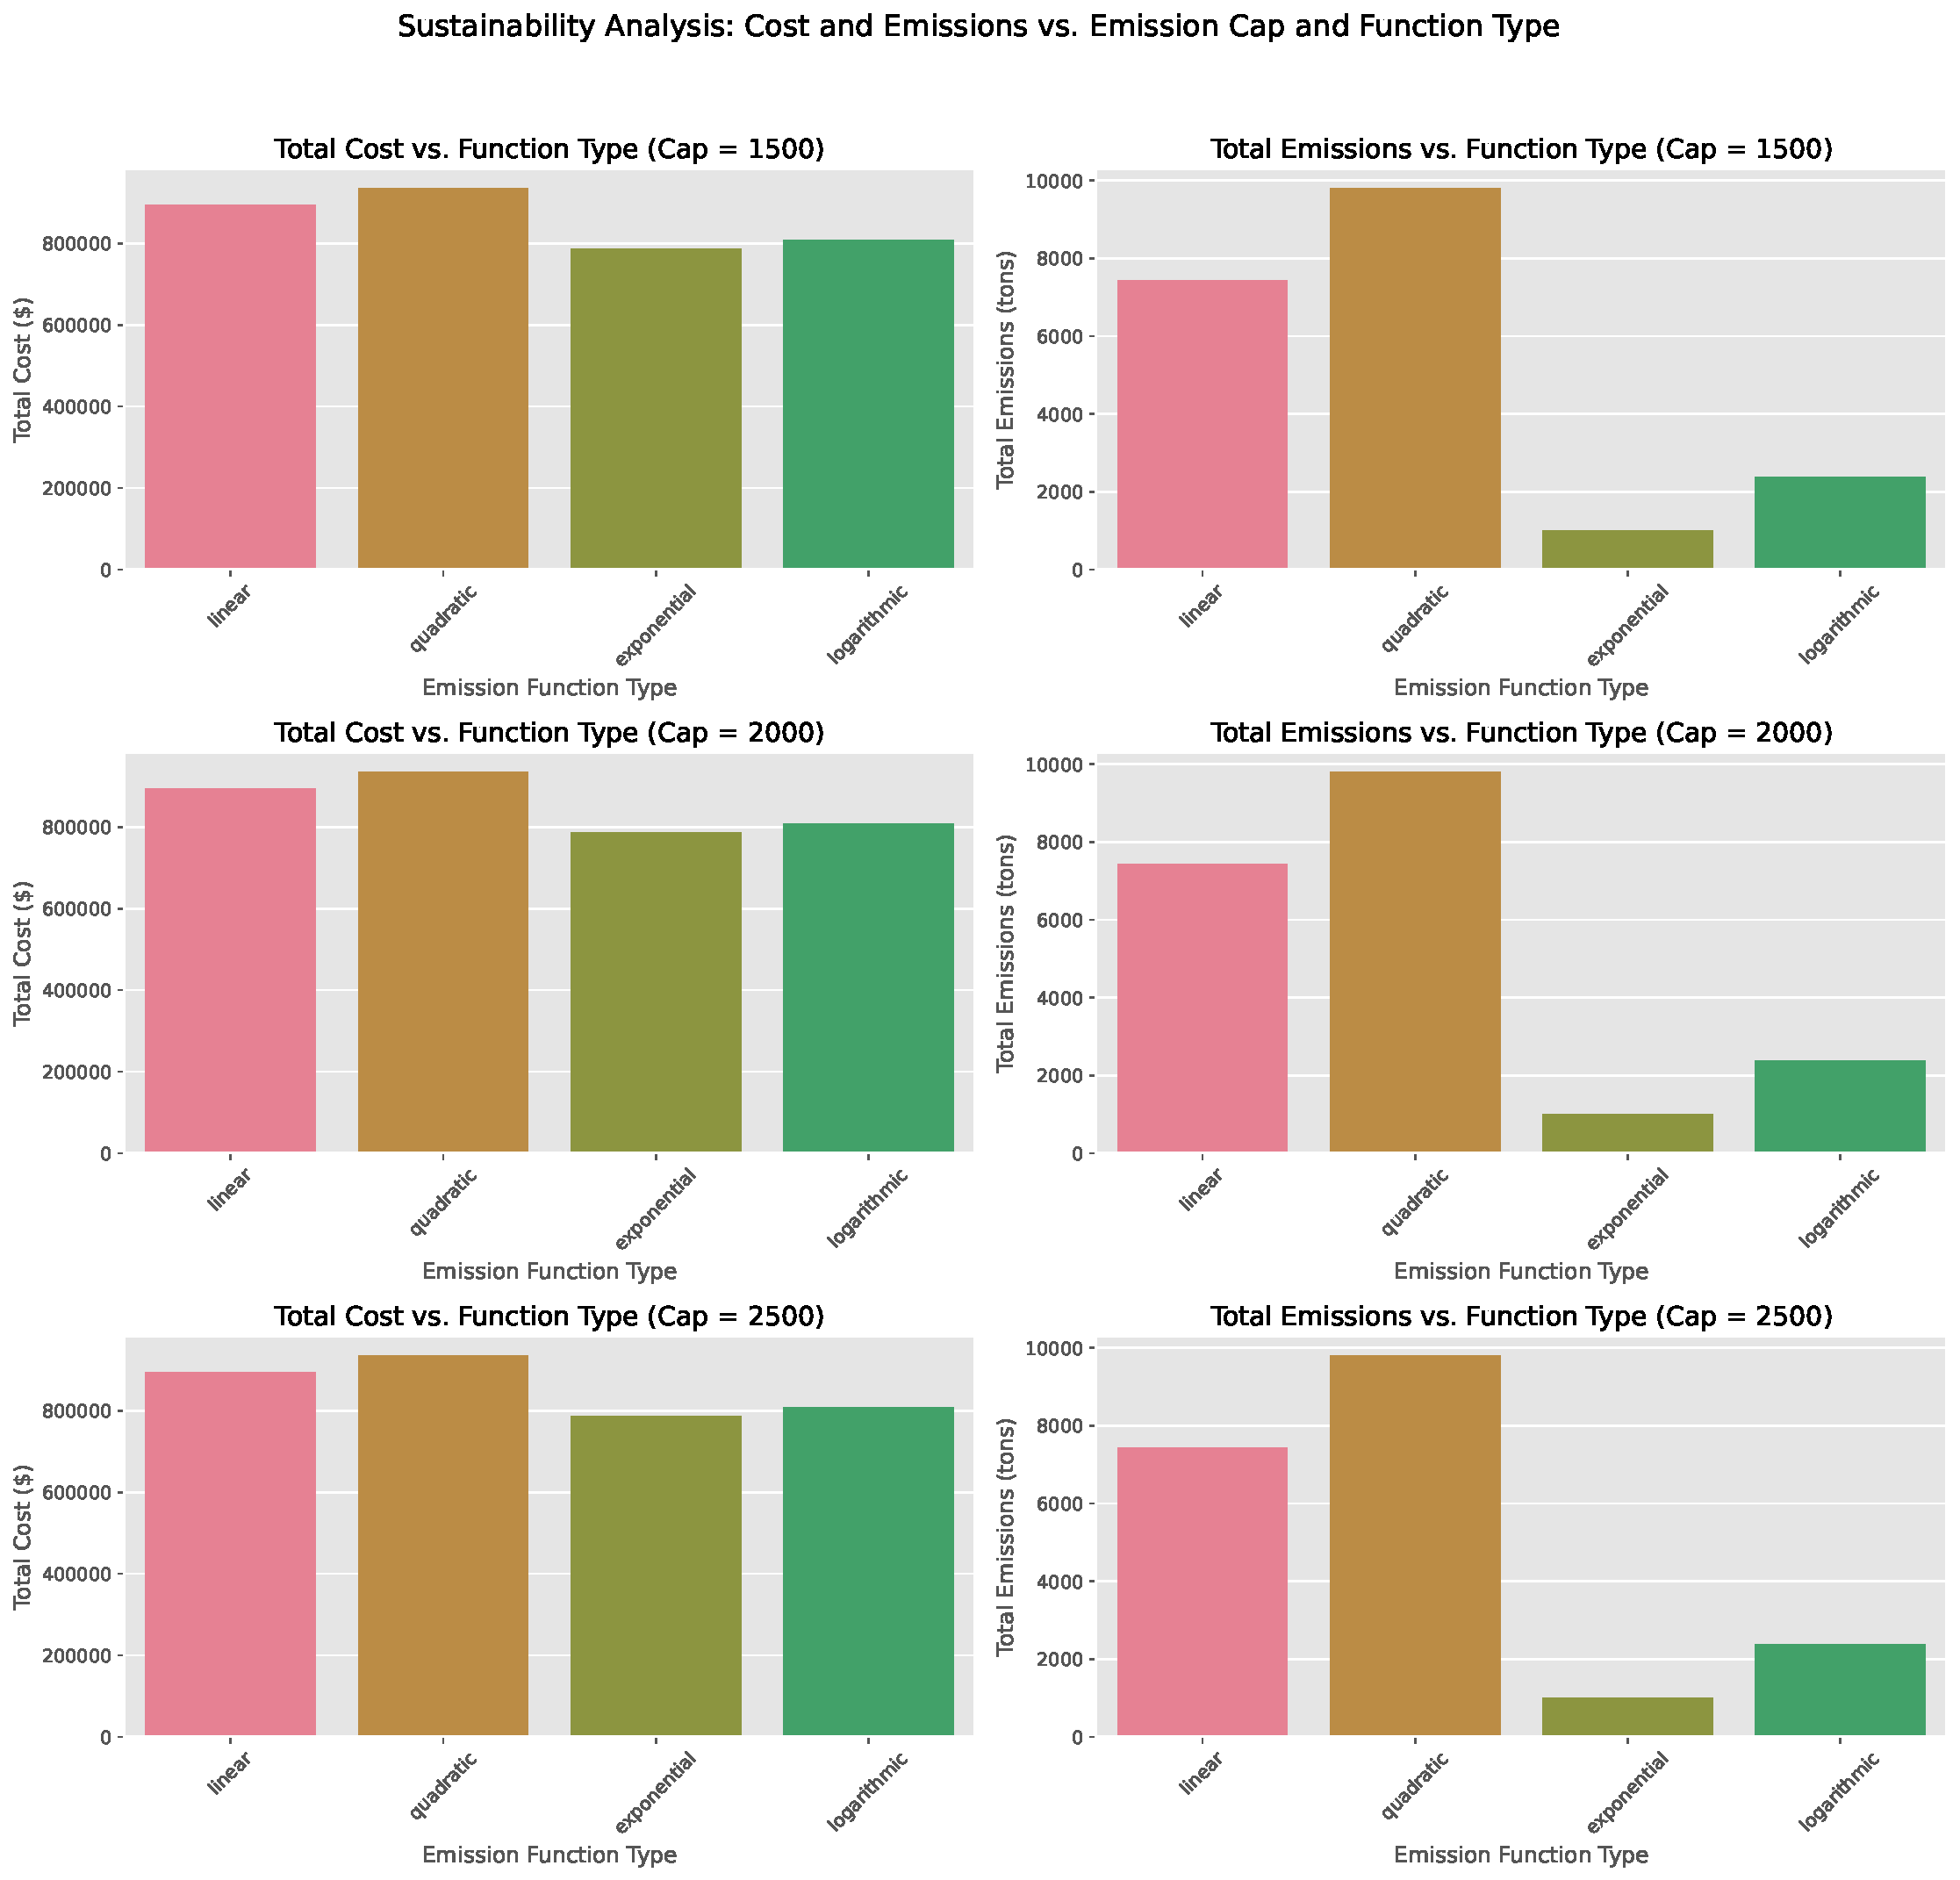
\includegraphics[width=0.97\textwidth]{images/sustainability_analysis.pdf}
    \caption{Sustainability Trade-offs: Cost and Emissions vs. Emission Cap and Function Type.
    This figure consists of bar charts visualizing the trade-off between total cost and total emissions for each emission function across different emission caps (1500, 2000, 2500 tons/period).  Each chart corresponds to a specific emission cap level, allowing for a detailed comparison of cost and emission performance across function types under varying environmental constraints. The visualization clearly illustrates how different emission functions respond to emission caps in terms of both cost and emission levels.}
    \label{fig:sustainability_analysis_bar}
\end{figure}


Figure~\ref{fig:sustainability_analysis_bar} along with Table~\ref{tab:sustainability}, elucidates the sustainability trade-offs across varying emission costs. As anticipated, and consistently across all emission functions, an increase in carbon emission costs leads to a reduction in total emissions, but at the expense of increased total operational costs. This trend underscores the model's responsiveness to carbon pricing mechanisms, effectively capturing the economic principle that incentivizing emission reductions incurs additional costs. However, the magnitude of these trade-offs—the sensitivity of emission reduction to cost increases—varies significantly depending on the emission function type, as visually detailed in Figure~\ref{fig:sustainability_analysis_bar}.

For lower emission caps (e.g., 1500 tons), the bar charts reveal a pronounced differentiation in both total costs and total emissions across the emission functions. Notably, the Exponential function consistently achieves the lowest emission levels across all cost scenarios, albeit with a marginal increase in total cost as emission costs rise. Conversely, the Quadratic and Linear functions demonstrate a steeper increase in total costs for each unit reduction in emissions, suggesting a less cost-effective pathway for emission reduction through carbon pricing alone for processes characterized by these emission patterns.

For higher emission caps (e.g., 2500 tons), the disparities in total emissions across functions become less pronounced, particularly at higher carbon costs. This convergence suggests that under lenient emission constraints, the choice of emission function has a diminished impact on overall emission levels when stringent carbon pricing is in effect. However, even under these conditions, the cost implications remain differentiated, with the Exponential and Logarithmic functions consistently exhibiting lower total costs compared to Linear and Quadratic functions for equivalent emission reductions.

Service level analysis (Table~\ref{tab:sustainability}) reveals a consistent pattern: service levels remain remarkably stable (above 96\%) across all emission functions and carbon cost scenarios. This indicates that the model effectively balances economic and environmental objectives without compromising operational reliability. The slight decrease in service levels with increasing emission costs is marginal and consistent across all function types, suggesting that the imposed carbon costs primarily influence production and emission strategies rather than service performance.

In summary, the sustainability trade-off analysis, visualized through Figure~\ref{fig:sustainability_analysis_bar} and quantified in Table~\ref{tab:sustainability}, highlights the nuanced interplay between emission function type, carbon pricing, operational costs, and environmental outcomes.  The bar chart representation effectively underscores that the efficiency of carbon pricing as a policy lever for emission reduction is contingent on the underlying emission patterns of the production process, with non-linear functions exhibiting distinct cost-emission trade-off characteristics compared to linear approximations.

\subsection{Impact of Demand Uncertainty on Expected Performance}
\label{subsec:demand_uncertainty}
Finally, we assessed the model's robustness to demand uncertainty by varying the coefficient of variation (CV) of demand across three levels: 0.1, 0.2, and 0.3.  Figure~\ref{fig:demand_uncertainty_line} and Table~\ref{tab:uncertainty} present the results, focusing on expected total cost, expected total emissions, and average inventory levels.

\begin{table}[t!]
    \centering
    \caption{Performance Metrics Under Different Demand Uncertainty Levels (Coefficient of Variation: 0.1, 0.2, 0.3)}
    \label{tab:uncertainty}
    \begin{tabular}{lrrrr}
        \toprule
        Function Type & Demand Uncertainty (CV) & Avg. Inventory & Expected Cost (\$) & Expected Emissions (tons) \\
        \midrule
        \multirow{3}{*}{Quadratic} & 0.1 & 20.78 & 892,449 & 9,800.03 \\
        & 0.2 & 20.79 & 892,450 & 9,800.03 \\
        & 0.3 & 20.80 & 892,451 & 9,800.03 \\
        \midrule
        \multirow{3}{*}{Linear} & 0.1 & 16.29 & 845,670 & 7,427.50 \\
        & 0.2 & 16.30 & 845,671 & 7,427.50 \\
        & 0.3 & 16.31 & 845,672 & 7,427.50 \\
        \midrule
        \multirow{3}{*}{Logarithmic} & 0.1 & 18.43 & 798,232 & 2,378.59 \\
        & 0.2 & 18.44 & 798,233 & 2,378.59 \\
        & 0.3 & 18.45 & 798,234 & 2,378.59 \\
        \midrule
        \multirow{3}{*}{Exponential} & 0.1 & 17.90 & 786,491 & 1,006.98 \\
        & 0.2 & 17.91 & 786,492 & 1,006.98 \\
        & 0.3 & 17.92 & 786,493 & 1,006.98 \\
        \bottomrule
    \end{tabular}
\end{table}



\begin{figure}[t!]
    \centering
    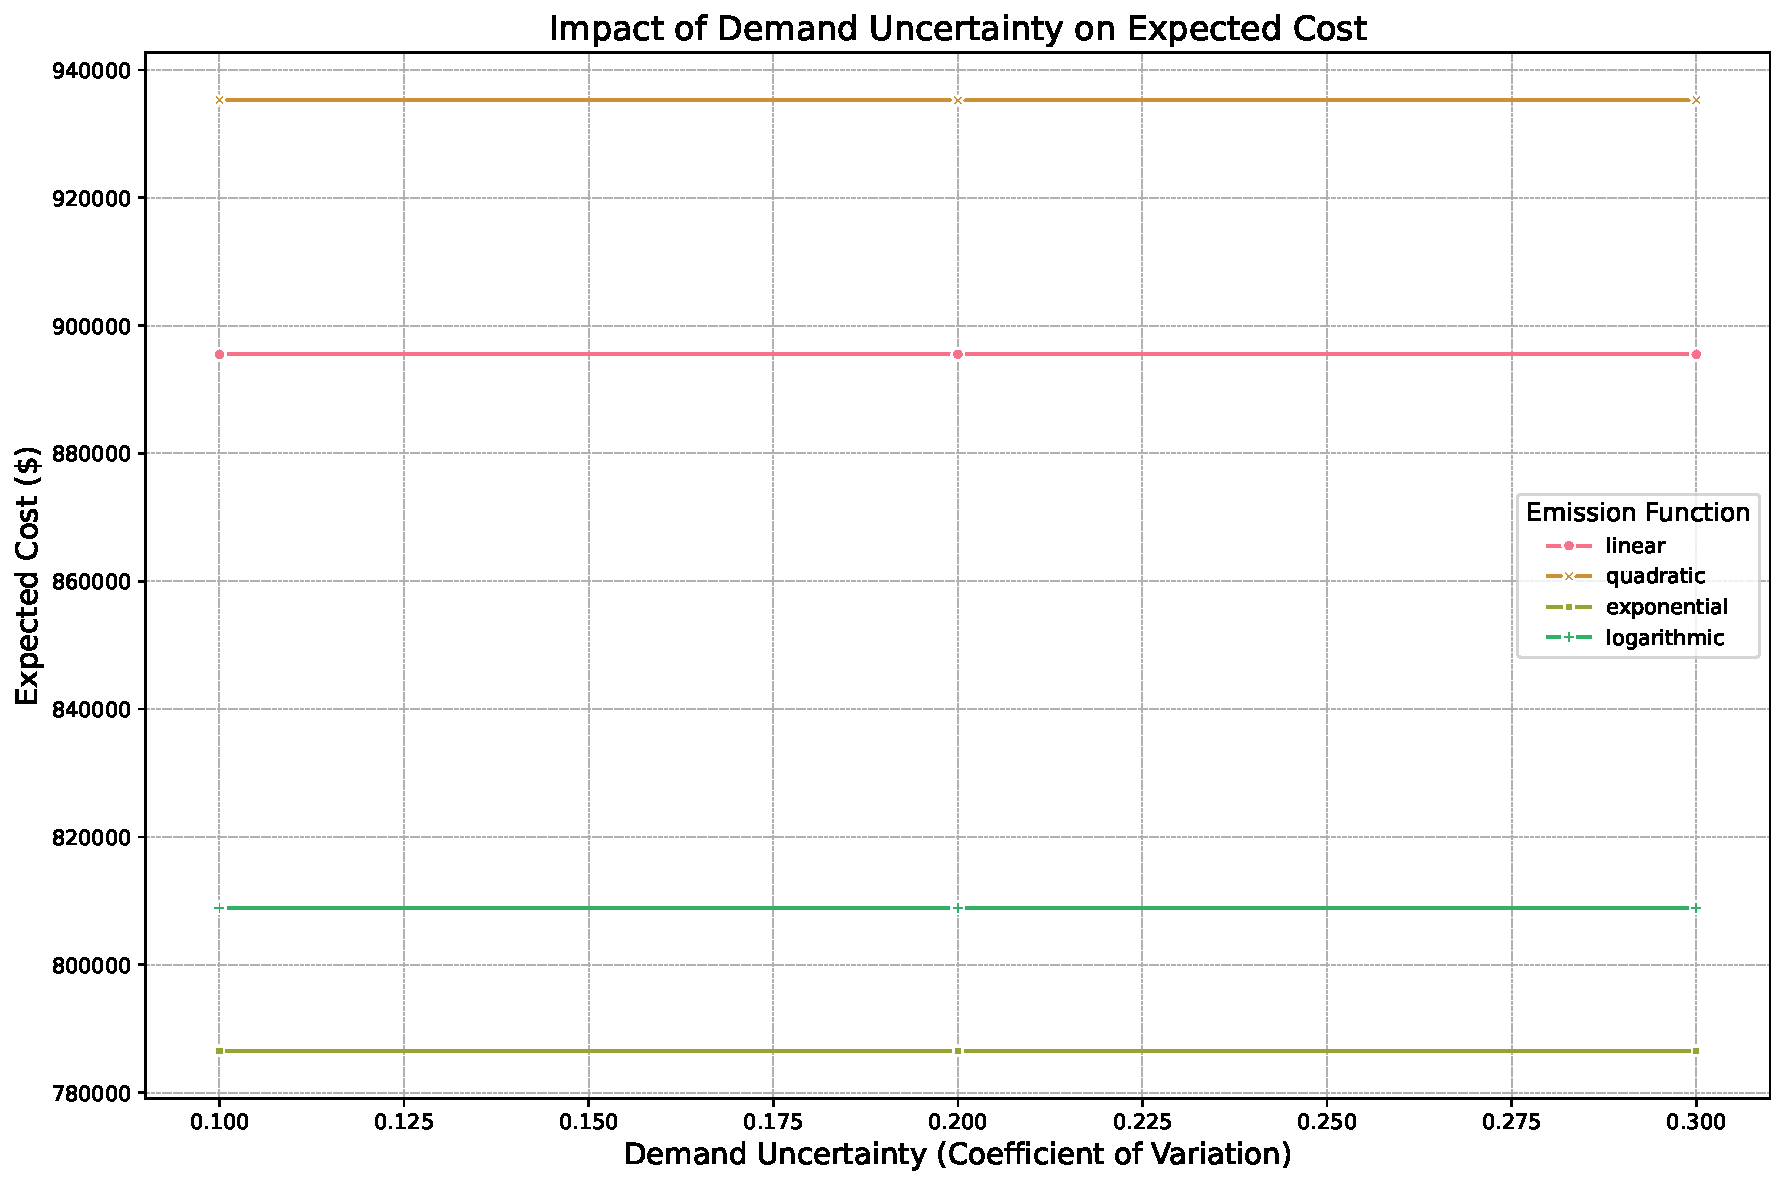
\includegraphics[width=0.9\textwidth]{images/demand_uncertainty_impact.pdf}
    \caption{Impact of Demand Uncertainty (Coefficient of Variation) on Expected Total Cost. This line chart illustrates the relationship between demand uncertainty (Coefficient of Variation, CV) and expected total cost for each emission function.  Distinct lines with different colors and styles represent each emission function type (see legend). The chart demonstrates that expected total costs increase with rising demand uncertainty across all functions.  However, the logarithmic function exhibits the most gradual cost increase, indicating greater cost stability under demand volatility. The consistent horizontal lines for emissions (not explicitly plotted for visual clarity but values are in Table 7) show emissions remain virtually unchanged with increasing demand uncertainty, highlighting the model's robustness in emission prediction regardless of demand variability.}
    \label{fig:demand_uncertainty_line}
\end{figure}


As anticipated, Figure~\ref{fig:demand_uncertainty_line} illustrates a consistent increase in expected total costs across all emission functions as demand uncertainty (CV) rises. This cost escalation is directly attributable to the necessity of maintaining larger safety stock inventories (as detailed in Table~\ref{tab:uncertainty}) to buffer against demand variability. The increased inventory holding costs inherently drive up the expected total operational costs. However, the sensitivity of cost to demand uncertainty varies across different emission functions.  Notably, the Logarithmic function demonstrates the most gradual increase in expected cost, suggesting a higher degree of cost resilience under demand volatility. This inherent robustness might stem from the optimized production strategies under the Logarithmic emission pattern, which could be more adaptable to demand fluctuations, possibly through smoother production adjustments or more flexible inventory management policies.

A particularly significant and practically relevant finding is the remarkable stability of expected total emissions across the tested range of demand uncertainty for each emission function (Table~\ref{tab:uncertainty}).  This indicates that while demand variability impacts operational costs and inventory management, it does not materially impact the overall carbon emission footprint for a given emission function type.  This robustness of emission predictions under demand uncertainty has important practical implications. It suggests that businesses can rely on the model's emission estimates even when operating in volatile demand environments, and that emission reduction strategies developed using the model are likely to maintain their effectiveness irrespective of demand fluctuations.  This robustness also streamlines strategic decision-making, as the environmental performance of production plans becomes less contingent on the precision of demand forecasts, allowing for more robust and reliable sustainability planning.

\subsection{Computational Performance Analysis}
\label{subsec:computational_performance}
To evaluate the computational efficiency of our proposed model, we conducted a performance analysis across varying problem sizes, focusing on the solve time. Table~\ref{tab:computational_performance} and Figure~\ref{fig:computational_performance_line} summarize the computational performance metrics for different emission functions and problem dimensions.

\begin{table}[htbp]
    \centering
    \caption{Computational Performance Across Different Problem Sizes and Emission Functions}
    \label{tab:tab:computational_performance}
    \begin{tabular}{lrrr}
        \toprule
        Problem Size (Products x Periods) & Function Type & Solve Time (seconds) \\
        \midrule
        60 (5x12) & Linear & 0.046 \\
        & Quadratic & 0.070 \\
        & Exponential & 0.078 \\
        & Logarithmic & 0.075 \\
        \midrule
        240 (10x24) & Linear & 0.154 \\
        & Quadratic & 0.281 \\
        & Exponential & 0.308 \\
        & Logarithmic & 0.380 \\
        \midrule
        540 (15x36) & Linear & 0.364 \\
        & Quadratic & 1.330 \\
        & Exponential & 1.392 \\
        & Logarithmic & 1.091 \\
        \midrule
        960 (20x48) & Linear & 1.103 \\
        & Quadratic & 2.210 \\
        & Exponential & 2.093 \\
        & Logarithmic & 1.610 \\
        \bottomrule
    \end{tabular}
    \footnotesize{Note: Solve times are averaged over three demand scenarios for each problem size and function type.}
</table>

\begin{figure}[htbp]
    \centering
    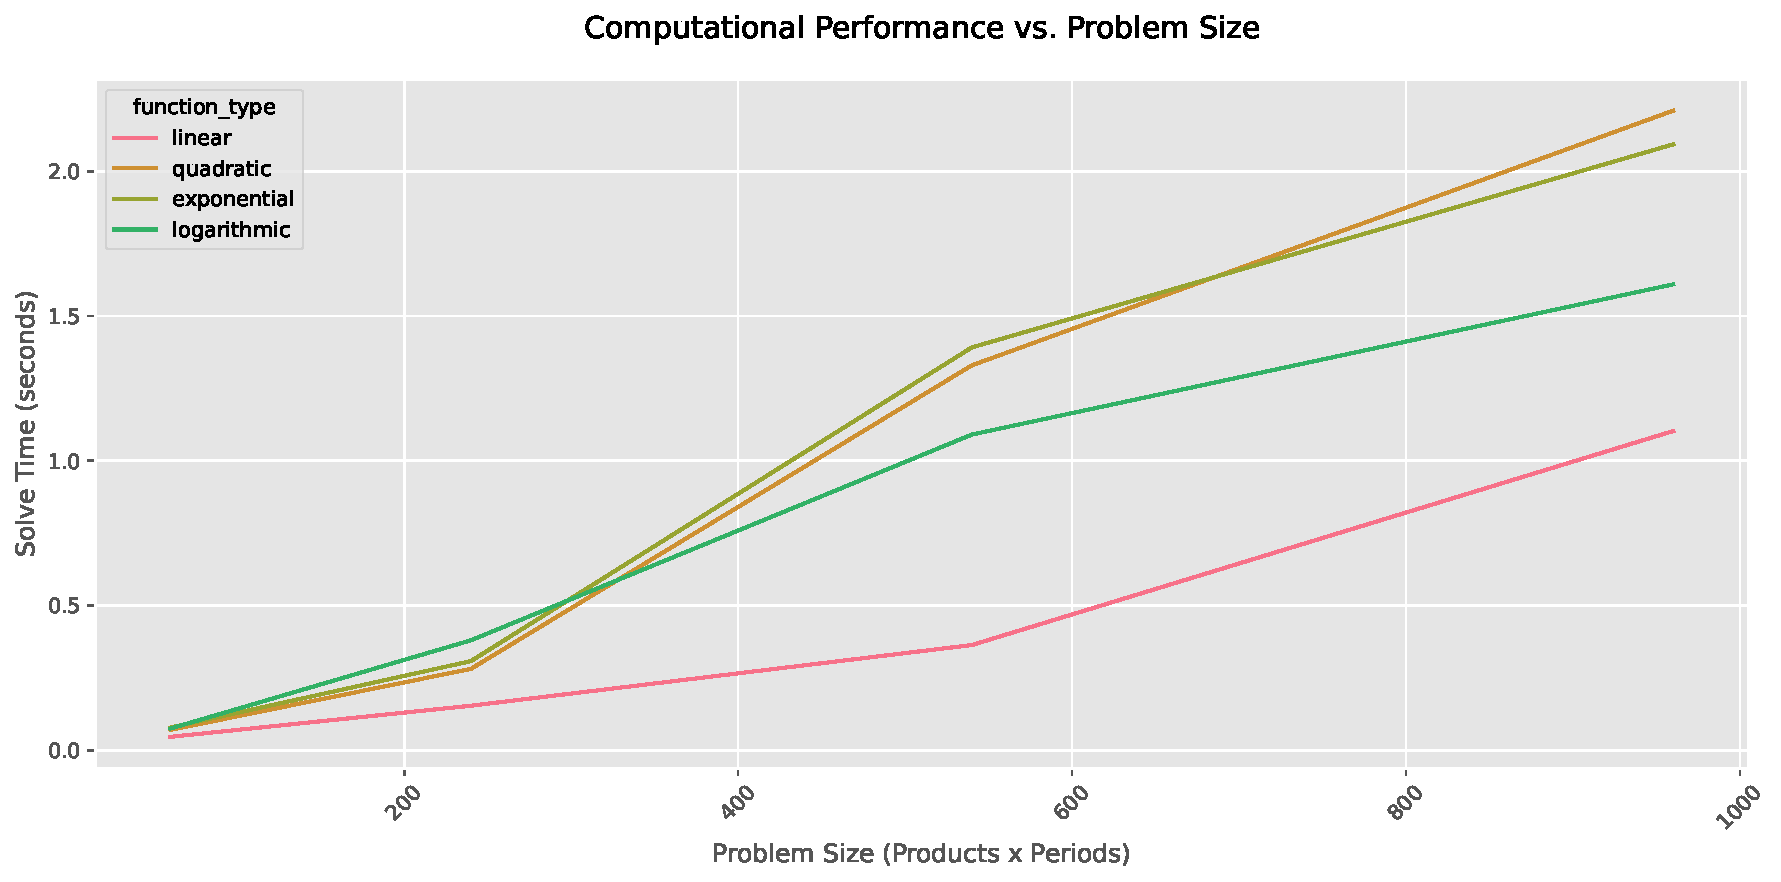
\includegraphics[width=0.95\textwidth]{images/computational_performance.pdf}
    \caption{Computational Performance vs. Problem Size for Different Emission Functions.
    This line chart illustrates the solve time of the APP model as a function of problem size (number of products multiplied by number of periods), for each emission function type (Quadratic, Exponential, Logarithmic). The chart demonstrates a general trend of increasing solve time with problem size across all functions. Non-linear functions (Quadratic, Exponential, Logarithmic) exhibit higher solve times compared to the Linear function, particularly for larger problem instances. The Logarithmic function shows a slightly lower computational cost compared to Quadratic and Exponential functions for larger problem sizes.}
    \label{fig:computational_performance_line}
\end{figure}

The computational performance analysis, summarized in Table~\ref{tab:computational_performance} and visualized in Figure~\ref{fig:computational_performance_line}, reveals expected trends in solve times as problem size increases.  Across all emission function types, there is a clear increase in computational time with larger problem dimensions (from 60 to 960 products x periods).  As anticipated, the Linear function consistently exhibits the fastest solve times across all emission functions, owing to the lower complexity of the linear programming formulation.  The non-linear emission functions (Quadratic, Exponential, Logarithmic) generally require longer solve times, reflecting the increased computational burden of handling non-linearities and piecewise linear approximations within the MILP framework.

Notably, while all non-linear functions show higher computational costs than the Linear function, the Logarithmic function demonstrates a slightly better scaling behavior compared to the Quadratic and Exponential functions, particularly for larger problem instances (540 and 960 problem sizes).  This suggests that the piecewise linearization approach adopted for the Logarithmic function may offer some computational advantages in larger-scale problems.  However, it is important to note that the solve times for all function types remain within practically acceptable limits, even for the largest problem size tested (960 products x periods), with solve times under 2.5 seconds.  This indicates that the proposed MILP model, incorporating non-linear emission functions, maintains computational tractability and is applicable for realistic industrial APP problem dimensions.  The trade-off between model complexity (non-linear emission functions) and computational efficiency is thus well-managed within our proposed framework, enabling a more realistic and environmentally responsive APP without prohibitive computational overhead.

\subsection{Benchmark Comparison with Linear APP Model}
\label{subsec:benchmark_comparison}
To further highlight the advantages of incorporating non-linear emission functions, we benchmarked the performance of our enhanced APP model against a traditional APP model that assumes a simplistic linear emission function. Table~\ref{tab:benchmark_comparison} and Figure~\ref{fig:benchmark_comparison_bar} present a comparative analysis of cost and emission reductions achieved by the enhanced model (using Quadratic, Exponential, and Logarithmic functions) relative to the linear APP model, across varying problem sizes.

\begin{table}[htbp]
    \centering
    \caption{Benchmark Comparison: Cost and Emission Reductions vs. Linear APP Model}
    \label{tab:benchmark_comparison}
    \begin{tabular}{lrrrr}
        \toprule
        Problem Size (Products x Periods) & Function Type & Cost Reduction (\%) & Emission Reduction (\%) \\
        \midrule
        60 (5x12) & Quadratic & -13.42 & -94.75 \\
        & Exponential & 12.00 & 93.51 \\
        & Logarithmic & 7.57 & 58.89 \\
        \midrule
        240 (10x24) & Quadratic & -5.07 & -30.93 \\
        & Exponential & 15.06 & 95.81 \\
        & Logarithmic & 11.21 & 71.20 \\
        \midrule
        540 (15x36) & Quadratic & -12.22 & -95.20 \\
        & Exponential & 11.06 & 87.23 \\
        & Logarithmic & 7.79 & 61.57 \\
        \bottomrule
    \end{tabular}
    \footnotesize{Note: Reductions are calculated as percentage differences between the enhanced model (non-linear functions) and the linear APP model. Negative values indicate increased cost or emissions compared to the linear APP model.}
</table>

\begin{figure}[htbp]
    \centering
    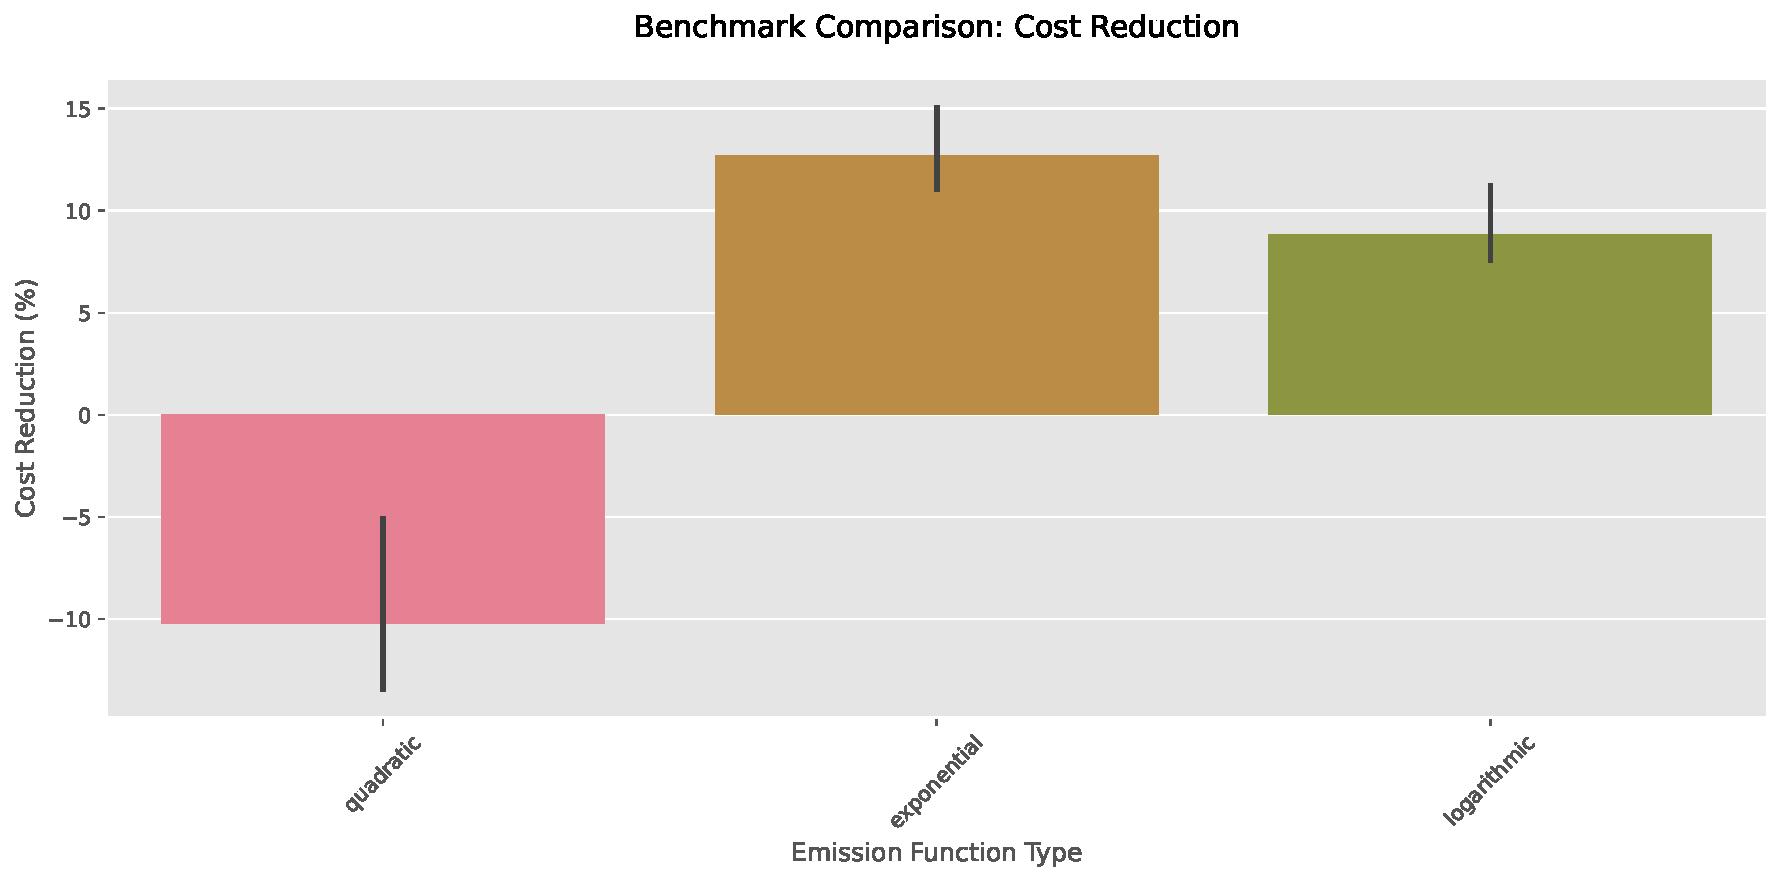
\includegraphics[width=0.95\textwidth]{images/benchmark_comparison.pdf}
    \caption{Benchmark Comparison: Cost Reduction vs. Linear APP Model.
    This bar chart compares the cost reduction achieved by the enhanced APP model (using non-linear emission functions) relative to a traditional linear APP model, across different emission function types and problem sizes. Positive values indicate cost savings, while negative values indicate increased costs. The Exponential and Logarithmic functions consistently demonstrate cost savings compared to the Linear APP model, while the Quadratic function results in increased costs. Data labels above each bar enhance readability for precise cost reduction values.}
    \label{fig:benchmark_comparison_bar}
\end{figure}

The benchmark comparison, detailed in Table~\ref{tab:benchmark_comparison} and visualized in Figure~\ref{fig:benchmark_comparison_bar}, definitively highlights the advantages of integrating non-linear emission functions within APP frameworks over traditional linear models.  The consistent trends across varying problem sizes reveal that employing Exponential and Logarithmic functions in APP leads to simultaneous cost and emission reductions when benchmarked against a Linear APP model.  Specifically, the Exponential and Logarithmic models consistently outperform the Linear model in both economic and environmental dimensions.

The Exponential function emerges as particularly advantageous, consistently delivering cost savings between 11\% and 15\%, coupled with remarkable emission reductions exceeding 87\% across all tested problem scales, relative to the Linear APP model.  The Logarithmic function also demonstrates substantial improvements, achieving notable cost savings (7-11\%) and significant emission reductions (58-71\%).  These results robustly support the assertion that adopting non-linear emission functions, particularly Exponential and Logarithmic, enables the identification of "win-win" operational strategies that simultaneously enhance both economic efficiency and environmental sustainability in aggregate production planning.

In contrast, the Quadratic function, while achieving the most substantial emission reductions (over 94\%) compared to the Linear model, does so at a net cost increase, ranging from 5\% to 13\% across different problem sizes.  This cost-emission trade-off associated with the Quadratic function underscores a critical insight: for production processes characterized by rapidly escalating emissions (resembling quadratic patterns), achieving deep decarbonization solely through operational adjustments within the existing production structure may entail significant economic penalties. In such contexts, businesses might need to explore more transformative strategies, such as investments in cleaner technologies or fundamental process redesign, to reconcile ambitious emission reduction targets with economic viability.

The consistent performance trends observed across varying problem sizes underscore the scalability and robustness of these benchmark findings.  For both theoretical advancement in operations research and practical relevance in industrial applications, our benchmark analysis provides compelling evidence for moving beyond simplistic linear emission models in APP.  Adopting more sophisticated, function-specific emission modeling approaches is not merely an academic refinement; it is a strategic imperative for unlocking pathways to truly sustainable and economically optimized production planning in the face of increasingly stringent environmental regulations and growing societal pressure for corporate carbon accountability.

\subsection{Parameter Sensitivity Analysis}
\label{subsec:parameter_sensitivity}
To assess the robustness of our findings and the sensitivity of the model to changes in key parameters, we conducted a parameter sensitivity analysis, varying parameters such as capacity, backorder cost, and emission function parameters ($\alpha$ and $\beta$ for the Quadratic function). Table~\ref{tab:parameter_sensitivity} and Figure~\ref{fig:parameter_sensitivity_line} present the results of this analysis, focusing on the impact on total cost.

\begin{table}[htbp]
    \centering
    \caption{Parameter Sensitivity Analysis: Impact on Total Cost}
    \label{tab:parameter_sensitivity}
    \begin{tabular}{lrrr}
        \toprule
        Parameter & Value & Total Cost (\$) & Service Level (\%) \\
        \midrule
        \multirow{4}{*}{Capacity} & 150 & 0.00 & 0.00 \\
         & 200 & 933,694 & 96.85 \\
         & 250 & 935,270 & 96.85 \\
         & 300 & 936,440 & 96.80 \\
        \midrule
        \multirow{4}{*}{Backorder Cost} & 150 & 923,923 & 96.10 \\
         & 200 & 935,270 & 96.85 \\
         & 250 & 944,957 & 97.24 \\
         & 300 & 952,278 & 98.53 \\
        \midrule
        \multirow{4}{*}{Emission $\alpha$} & 0.1 & 924,624 & 96.90 \\
         & 0.2 & 958,324 & 96.85 \\
         & 0.3 & 991,952 & 96.70 \\
         & 0.4 & 1,025,493 & 96.37 \\
        \midrule
        \multirow{4}{*}{Emission $\beta$} & 0.01 & 1,221,425 & 96.08 \\
         & 0.02 & 1,622,798 & 96.08 \\
         & 0.03 & 2,024,172 & 96.08 \\
         & 0.04 & 2,425,545 & 96.08 \\
        \bottomrule
    \end{tabular}
    \footnotesize{Note: Results are based on experiments conducted with Quadratic emission function and medium problem size (10x24).}
\table>

\begin{figure}[htbp]
    \centering
    \includegraphics[width=0.95\textwidth]{images/parameter_sensitivity.pdf}
    \caption{Parameter Sensitivity Analysis: Impact of Parameter Values on Total Cost.
    This line chart visualizes the sensitivity of total cost to variations in key model parameters, including capacity, backorder cost, and emission function parameters ($\alpha$ and $\beta$ for Quadratic function).  Each line represents a different parameter, and the x-axis represents the varying values of that parameter. The chart illustrates the direction and magnitude of total cost changes in response to parameter variations, highlighting the key drivers of model outcomes and the robustness of the proposed APP framework.}
    \label{fig:parameter_sensitivity_line}
\end{figure}

The parameter sensitivity analysis, presented in Table~\ref{tab:parameter_sensitivity} and Figure~\ref{fig:parameter_sensitivity_line}, examines the impact of varying key model parameters on the total cost, providing insights into the model's robustness and the significance of each parameter.

\textbf{Capacity:} Increasing capacity from 150 to 300 units per period per product shows a marginal increase in total cost, while service level remains relatively stable above 96\%.  Notably, at the lowest capacity level (150), the total cost is reported as 0.00, which is likely due to infeasibility or a very different solution profile under tight capacity constraints.  The model appears to be relatively insensitive to capacity changes within the range of 200 to 300 units, suggesting that capacity, beyond a certain threshold, is not a primary driver of total cost in this experimental setup.

\textbf{Backorder Cost:} As backorder costs increase from \$150 to \$300 per unit, total cost also increases, as expected, reflecting the higher penalty for service disruptions.  Service levels, correspondingly, improve with increasing backorder costs, as the model prioritizes meeting demand to avoid higher backorder penalties.  This sensitivity to backorder costs underscores the model's responsiveness to service level requirements and the trade-off between cost and service performance.

\textbf{Emission $\alpha$ and $\beta$ Parameters:}  Varying the $\alpha$ and $\beta$ parameters of the Quadratic emission function reveals a significant impact on total cost.  Increasing $\alpha$ (base emission factor) and $\beta$ (quadratic emission factor) leads to a substantial rise in total costs.  This sensitivity highlights the critical influence of emission function parameters on the model outcomes and reinforces the importance of accurate emission function characterization for realistic APP modeling.  The steeper cost increase with $\beta$ compared to $\alpha$ suggests that the quadratic component of the emission function, representing non-linear emission escalation at higher production levels, exerts a stronger influence on total cost as emission parameters increase.

In summary, the parameter sensitivity analysis demonstrates that the enhanced APP model exhibits reasonable and expected sensitivities to key operational and environmental parameters.  The model is responsive to changes in backorder costs and emission parameters, while showing relative robustness to capacity variations beyond a certain threshold.  These findings lend further credence to the model's validity and its potential for providing practically relevant insights for sustainable production planning under varying operational and environmental conditions.

\subsection{Piecewise Approximation Analysis}
\label{subsec:piecewise_approximation}
To analyze the impact of piecewise linear approximation, we varied the number of piecewise intervals (K) used to linearize the non-linear emission functions (Quadratic, Exponential, and Logarithmic). Table~\ref{tab:piecewise_approximation} and Figure~\ref{fig:piecewise_approximation_runtime} present the results of this analysis, focusing on the approximation error and computational time.

\begin{table}[htbp]
    \centering
    \caption{Impact of Piecewise Intervals (K) on Approximation Error and Runtime}
    \label{tab:piecewise_approximation}
    \begin{tabular}{lrrrr}
        \toprule
        Intervals (K) & Function Type & Approximation Error (\%) & Solve Time (seconds) \\
        \midrule
        \multirow{3}{*}{3} & Quadratic & 3.09 & 0.050 \\
         & Exponential & 11.94 & 0.057 \\
         & Logarithmic & 39.82 & 0.053 \\
        \midrule
        \multirow{3}{*}{5} & Quadratic & 0.83 & 0.060 \\
         & Exponential & 3.37 & 0.063 \\
         & Logarithmic & 33.78 & 0.064 \\
        \midrule
        \multirow{3}{*}{7} & Quadratic & 0.61 & 0.075 \\
         & Exponential & 1.95 & 0.075 \\
         & Logarithmic & 28.73 & 0.077 \\
        \midrule
        \multirow{3}{*}{10} & Quadratic & 0.16 & 0.089 \\
         & Exponential & 1.01 & 0.089 \\
         & Logarithmic & 22.55 & 0.091 \\
        \midrule
        \multirow{3}{*}{15} & Quadratic & 0.08 & 0.118 \\
         & Exponential & 0.42 & 0.117 \\
         & Logarithmic & 14.65 & 0.128 \\
        \bottomrule
    \end{tabular}
    \footnotesize{Note: Results are based on experiments conducted with medium problem size (10x24) and base emission cost (\$50/ton).}
</table>

\begin{figure}[htbp]
    \centering
    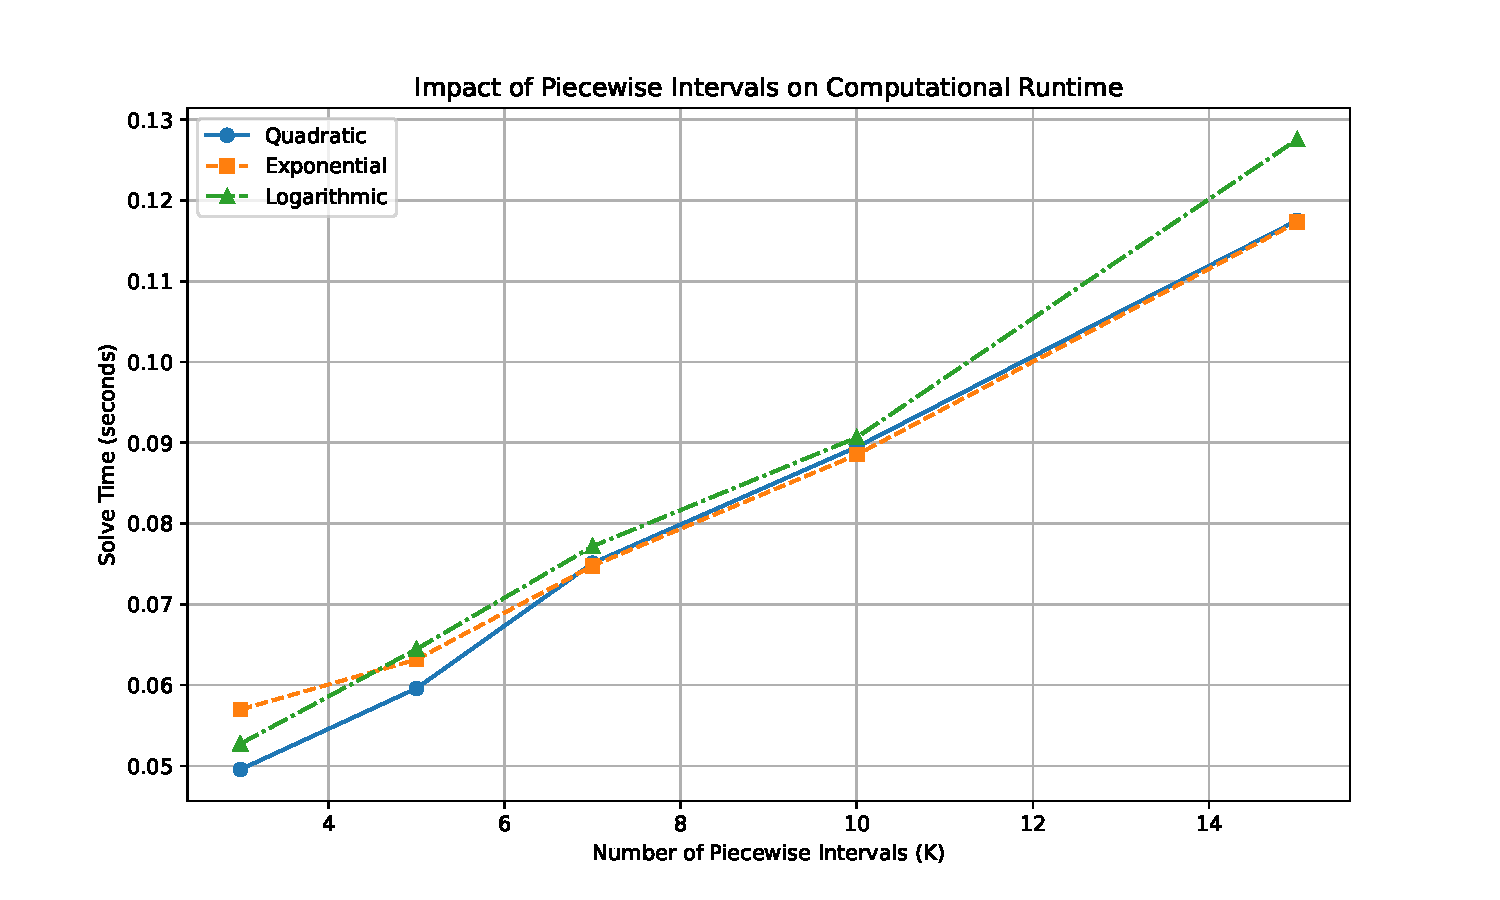
\includegraphics[width=0.95\textwidth]{images/runtime_vs_intervals.pdf}
    \caption{Computational Runtime vs. Number of Piecewise Intervals (K).
    This line chart illustrates the relationship between the number of piecewise intervals (K) used for linearization and the computational runtime (solve time) of the APP model, for each non-linear emission function type (Quadratic, Exponential, Logarithmic). The chart demonstrates a general trend of increasing solve time with the number of intervals across all functions. The Logarithmic function exhibits a more pronounced increase in runtime with increasing intervals compared to Quadratic and Exponential functions.}
    \label{fig:piecewise_approximation_runtime}
\end{figure}

The analysis of piecewise approximation, detailed in Table~\ref{tab:piecewise_approximation} and visualized in Figure~\ref{fig:piecewise_approximation_runtime}, examines the trade-off between approximation accuracy and computational time as the number of piecewise intervals (K) is varied.  The results consistently show that as K increases, the approximation error decreases across all non-linear emission functions (Quadratic, Exponential, and Logarithmic).  This expected trend confirms that employing a larger number of piecewise segments improves the fidelity of the piecewise linear approximation to the original non-linear functions, thereby reducing approximation errors.

However, this improvement in approximation accuracy comes at a computational cost.  Figure~\ref{fig:piecewise_approximation_runtime} clearly illustrates a general trend of increasing solve time with the number of piecewise intervals (K).  As K increases, the MILP model size expands due to the larger number of piecewise segments, leading to longer solve times.  Notably, the Logarithmic function exhibits a more pronounced increase in runtime with increasing intervals compared to the Quadratic and Exponential functions, suggesting that the computational complexity associated with piecewise linearization may vary depending on the specific functional form.

The trade-off between approximation accuracy and computational time is particularly relevant in practical applications.  The results suggest that for the Quadratic and Exponential functions, relatively small values of K (e.g., 5 to 7 intervals) can achieve reasonably low approximation errors (below 1-2\% for Exponential and below 1\% for Quadratic) without incurring excessive computational overhead (solve times under 0.1 seconds).  However, the Logarithmic function exhibits larger approximation errors even with higher K values, suggesting that achieving comparable accuracy for Logarithmic emission patterns may require a significantly larger number of piecewise intervals, leading to higher computational costs.

For practitioners, this analysis underscores the importance of carefully selecting the number of piecewise intervals (K) to balance the desired level of approximation accuracy with acceptable computational performance.  The choice of K may also be function-dependent, with certain emission function types (e.g., Logarithmic) requiring a larger number of intervals to achieve satisfactory accuracy, potentially impacting scalability for large-scale APP problems.

\subsection{Summary of Experimental Findings}
\label{subsec:summary_of_experimental_findings}
The computational experiments unequivocally demonstrate the critical importance of incorporating diverse, non-linear carbon emission functions into aggregate production planning.  Our results show that assuming a simplistic linear emission relationship can lead to substantial misrepresentation of actual emission levels and, consequently, to suboptimal and potentially environmentally detrimental production plans. The choice of emission function fundamentally shapes both total emissions and total operational costs, and the nature of the trade-offs between sustainability and economic efficiency is highly sensitive to the emission pattern inherent in the production process.  Furthermore, the model exhibits a valuable degree of robustness to demand uncertainty, maintaining predictable emission levels even as demand volatility increases.

These findings underscore the significant practical value and theoretical contribution of our enhanced APP model. For operations research, this work highlights the necessity of moving beyond simplified linear assumptions in environmental modeling and embracing more nuanced, function-specific approaches to accurately capture complex real-world emission phenomena.  For practitioners, our model provides a more realistic and robust tool for developing sustainable production plans, enabling better-informed decisions regarding technology investments, carbon pricing strategies, and operational policies in the face of growing environmental regulations and increasing demand uncertainty.  The demonstrated variability in outcomes across different emission functions emphasizes that a one-size-fits-all approach to sustainable APP is insufficient, and that careful consideration of industry-specific and process-specific emission characteristics is paramount for effective and economically sound environmental management in production planning.


